Several previous authors have used the GEANT4 toolkit to simulate the light collection efficiency of their detector designs.
In PNNL 14283 the authors looked at a variety of different PMT placement and detectors designs to increase the light output of a detector in the Advanced Large-Area Plastic Scintillators (ALPS) project \cite{pnnl_14283}.
The authors found that for a \SI{127}{\cm} by \SI{57}{\cm} by \SI{5}{\cm} slab of BC-408 wrapped in a loose foil of 85\% reflectivity that the light output could be almost doubled by doubling the number of PMT's.
These results are summarized in \autoref{tab:PNNLLightCollectionEfficiency}.
\begin{table}
  \centering
  \caption[PNNL Light Collection Efficiencies]{Light collection efficiencies of several detector designs simulated by PNNL\cite{pnnl_14283}.}
  \label{tab:PNNLLightCollectionEfficiency}
  \begin{tabular}{c|c c}
  \toprule
  & \multicolumn{2}{c}{Light Collection Efficiency} \\
  Number of PMTs  & 2-in PMT & 5-in PMT \\
  \midrule
  2 & 7.0\% & 18.8\% \\
  4 & 13.3\% & 30.7\ \\
  6 & 18.4\% & 40.2\% \\
  \bottomrule
  \end{tabular}
\end{table}
In addition, other authors have reported on the simulation performance of a light guides and photon attenuation using the GEANT4 toolkit.

This design has the \SI{100}{\um}, 10\% loaded \iso[6]{LiF} films sandwiched between wavelength shifting (each \SI{5}{\mm} thick) with a single PMT at the top and bottom.
This design collects 8\% of the optical photons emitted; for a polystyrene film with an average light yield of 2,000 photons per neutron 400 would then hit the photocathode.
It is expected that this is enough photons to create a signal above the noise for a typical PMT.
\begin{figure}
  \centering
	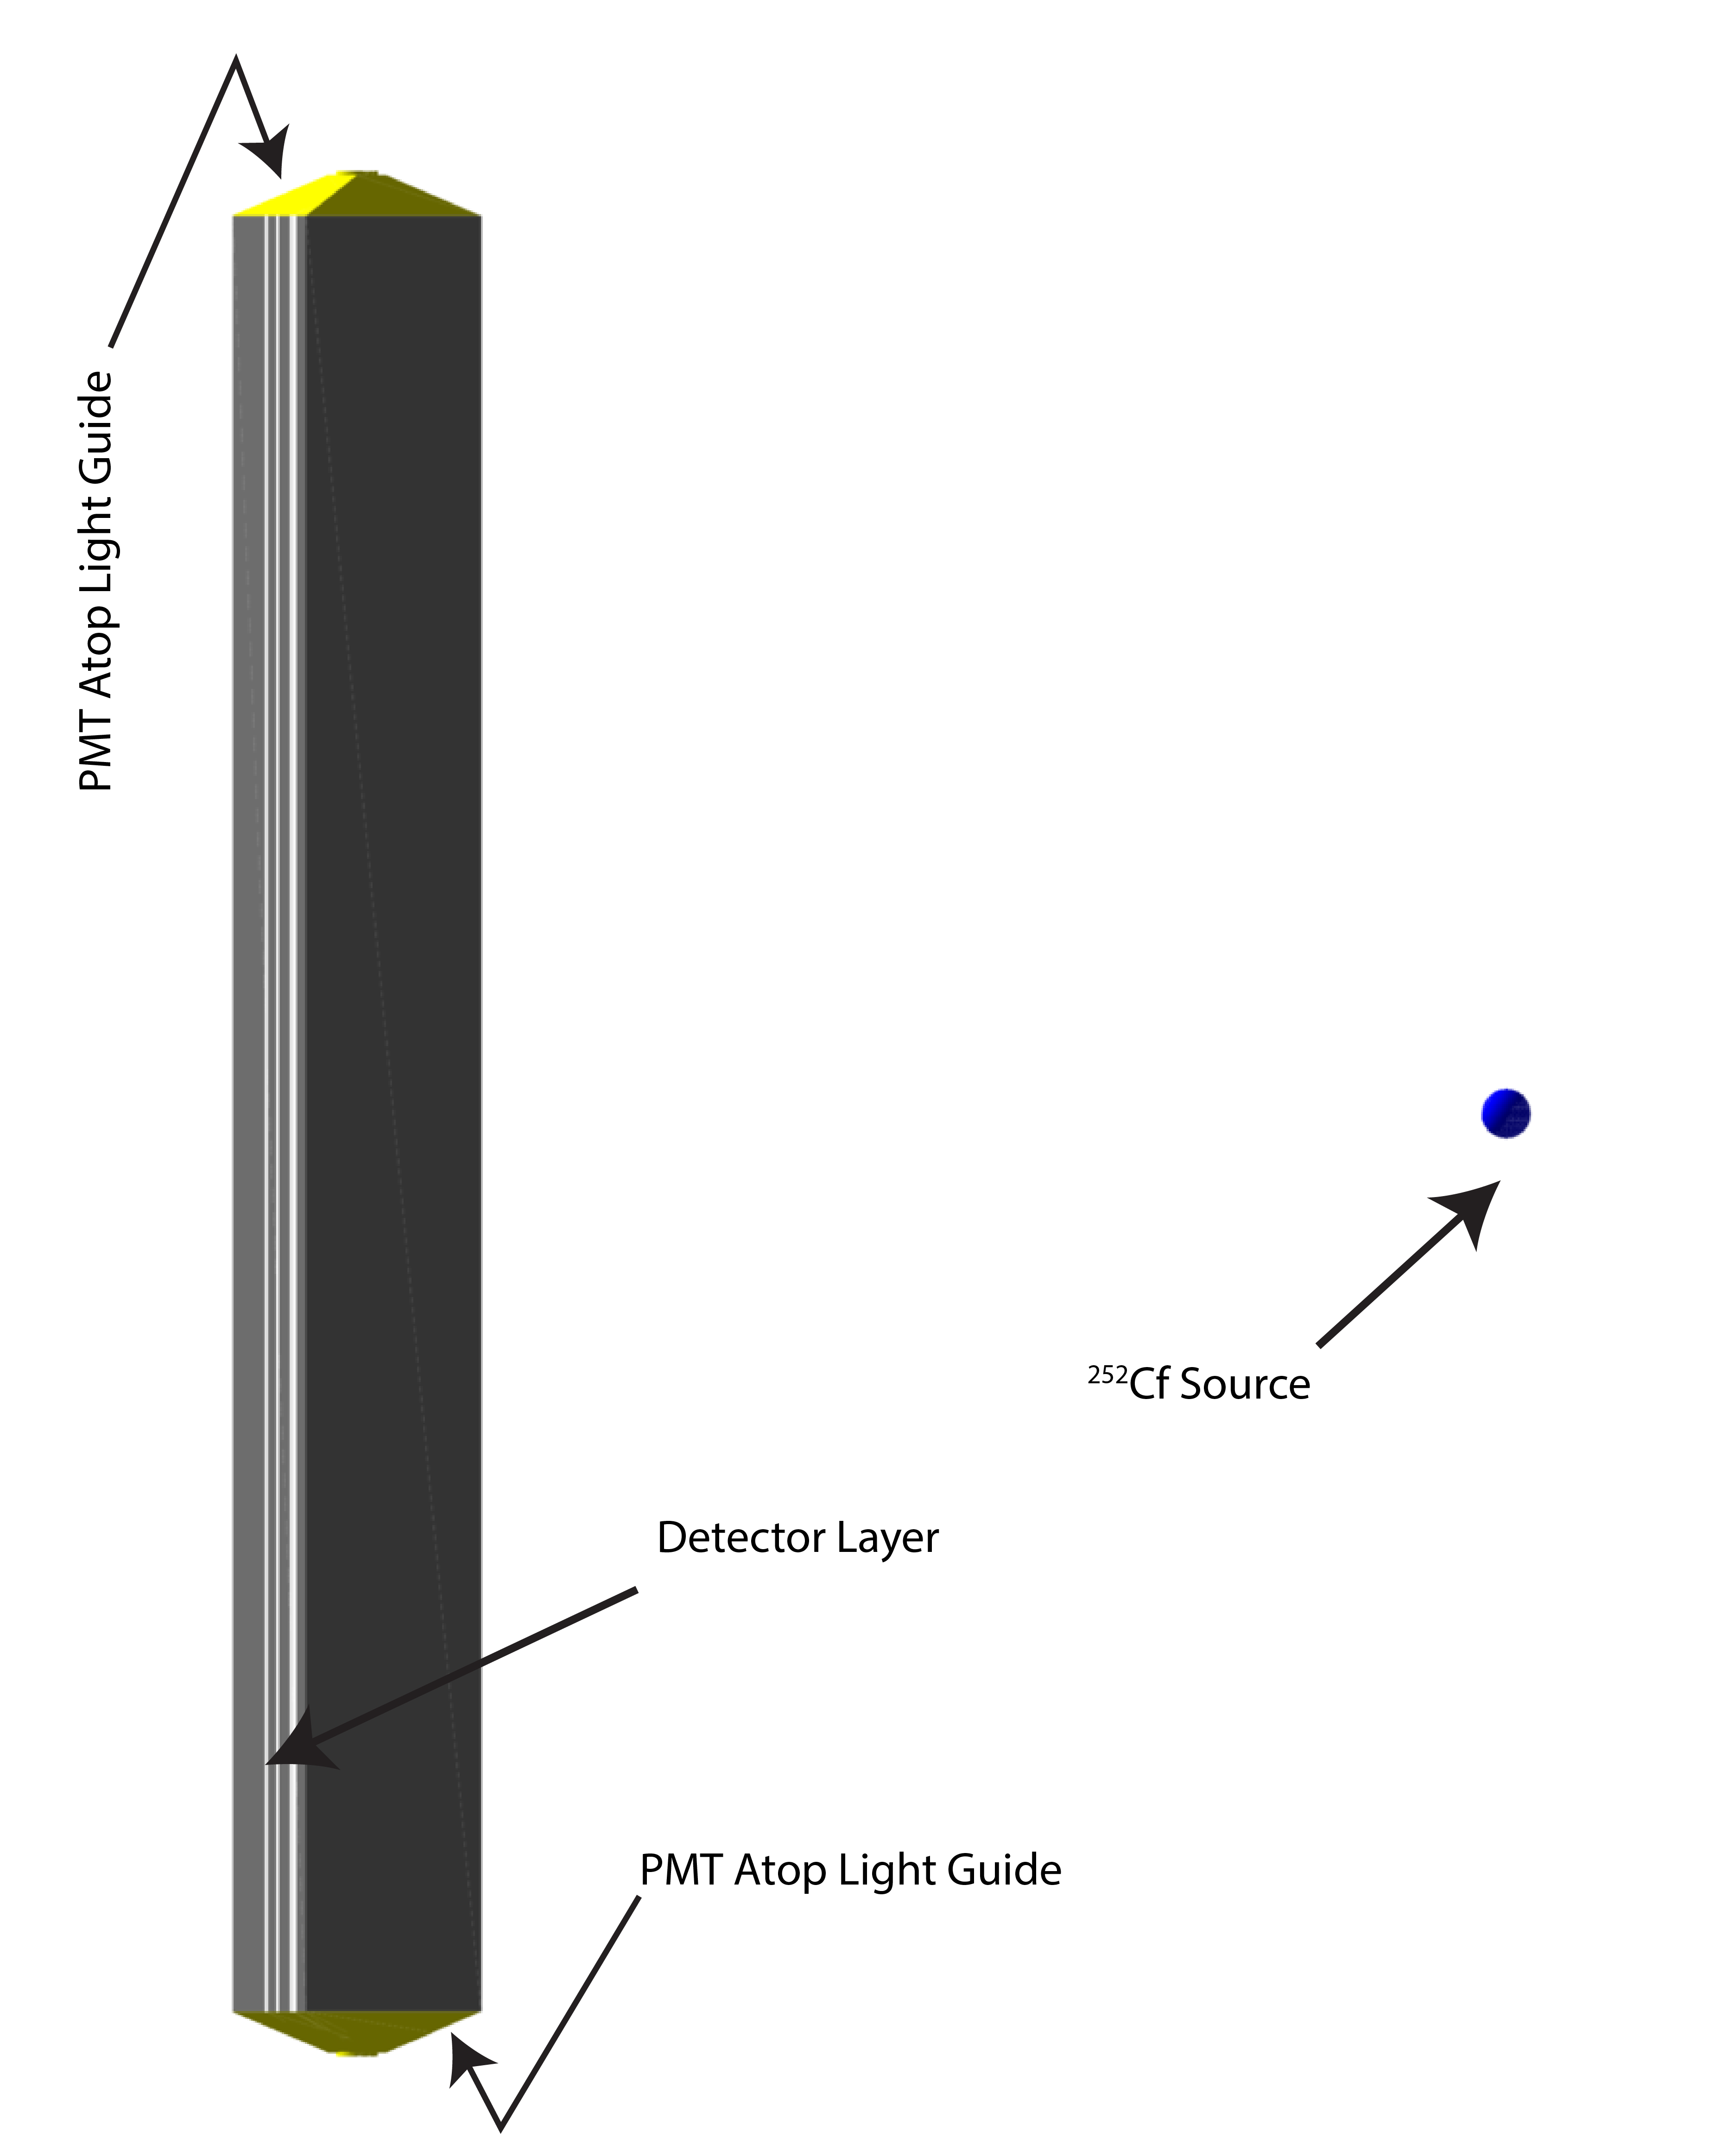
\includegraphics[width=\textwidth]{GEANT4AnnotatedGeo_RPM8SimGeo}
	  \caption[GEANT4 Simulated RPM8 Detector Design]{Simulated RPM8 with light transport in GEANT4. This design is capable of meeting all of the criteria set forth for radiation portal monitors.}
  \label{fig:G4RPM8Geo}
\end{figure}


Different cladding coatings were studied for their effect on the collection efficiency of a scintillator.
The collection efficiencies are presented in \autoref{tab:CladStudy}.
\begin{table}
  \caption[Teflon, Mylar, and HDPE Cladding Light Collection Effect]{The effect of Teflon, mylar, and HDPE cladding on the light collection of a scintillating slab}.
  \label{tab:CladStudy}
  \begin{tabular}{p{4cm} m{3cm} m{3cm}}
  \toprule
  & Coating & Fraction of Photons Collected \\
  \midrule 
  \multirow{3}{*}{EJ-200} & Teflon & 12\% \\
  				      & Air &  14\% \\
				      & Mylar & 9.6\% \\
  \midrule 
  \multirow{3}{*}{PS LiF} & Teflon & 4.3\% \\
  				      & Air & 4.5\% \\
				      & Mylar & 4.0\% \\
  \midrule 
  \multirow{3}{*}{EJ-426} & Teflon & \num{4.6E-3}\% \\
  				      & Air & \num{4.5E-3}\% \\
				      & Mylar & \num{4.2E-3}\% \\
 \bottomrule				 	   				  
  \end{tabular}
\end{table}
  \begin{table}
  \caption[Light Collection Increase with a WLS Bar]{Effect of a WLS on the light collection of a scintillating slab.}
  \label{tab:WLSStudy}
  \begin{tabular}{p{4cm} m{3cm} m{3cm}}
  \toprule
  & \multicolumn{2}{c}{Precent Photons Detected} \\
  Detector Material & PMMA &  WLS \\
  \midrule
 EJ-200 & 0.68\%  & 12\% \\
 PS LiF & 0.14\% & 4.3\% \\
 EJ-426 & \num{1.3E-3}\% & \num{4.5E-3}\% \\
 \bottomrule
  \end{tabular}
\end{table}

%An overview of the light transport and scintillation processes available in GEANT4 is presented in \cite{riggi_introducing_2011}.
%The authors also simulated a \SI{1}{\m} by \SI{1}{\cm} by \SI{1}{\cm} plastic strip in order to calculate the photon attenuation in the plastic.
%Two orders of magnitude drop in the number of photons was calculated for photons collected \SI{90}{\cm} from the distance of emission, and was highly dependent of the reflectivity of the material encasing the plastic strip\cite{riggi_introducing_2011}.
%Polymeric detectors containing PPO/POPOP as the fluor have also been modeled for the light transport with GEANT4\cite{5485130}.

MeasLayeredDetector_EJ426Mounting.png
MeasLayeredDetector_MountingLayers.png
